%%%%%%%%%%%%%%%%%%%%%%%%%%%%%%%%%%%%%%%%%
% Short Sectioned Assignment
% LaTeX Template
% Version 1.0 (5/5/12)
%
% This template has been downloaded from:
% http://www.LaTeXTemplates.com
%
% Original author:
% Frits Wenneker (http://www.howtotex.com)
%
% License:
% CC BY-NC-SA 3.0 (http://creativecommons.org/licenses/by-nc-sa/3.0/)
%
%%%%%%%%%%%%%%%%%%%%%%%%%%%%%%%%%%%%%%%%

%----------------------------------------------------------------------------------------
%	PACKAGES AND OTHER DOCUMENT CONFIGURATIONS
%----------------------------------------------------------------------------------------

\documentclass[paper=a4, fontsize=12pt, xcolor=dvipsnames]{scrartcl} % A4 paper and 11pt font size

% Biblatex

\usepackage[
style=nature,    % Zitierstil
isbn=false,                % ISBN nicht anzeigen, gleiches geht mit nahezu allen anderen Feldern
pagetracker=true,          % ebd. bei wiederholten Angaben (false=ausgeschaltet, page=Seite, spread=Doppelseite, true=automatisch)
maxbibnames=50,            % maximale Namen, die im Literaturverzeichnis angezeigt werden (ich wollte alle)
maxcitenames=3,            % maximale Namen, die im Text angezeigt werden, ab 4 wird u.a. nach den ersten Autor angezeigt
autocite=inline,           % regelt Aussehen für \autocite (inline=\parancite)
block=space,               % kleiner horizontaler Platz zwischen den Feldern
backref=false,              % Seiten anzeigen, auf denen die Referenz vorkommt
backrefstyle=three+,       % fasst Seiten zusammen, z.B. S. 2f, 6ff, 7-10
date=short,                % Datumsformat
backend = bibtex
]{biblatex}
\setlength{\bibitemsep}{1em}     % Abstand zwischen den Literaturangaben
\setlength{\bibhang}{2em}        % Einzug nach jeweils erster Zeile
\bibliography{report}  % Bibtex-Datei wird schon in der Preambel eingebunden

\usepackage[T1]{fontenc} % Use 8-bit encoding that has 256 glyphs
\usepackage{fourier} % Use the Adobe Utopia font for the document - comment this line to return to the LaTeX default
\usepackage{amsmath,amsfonts,amsthm} % Math packages
\usepackage{pgfplots}
\usepackage{wrapfig}
\usepackage{sidecap}
\usepackage{color, colortbl}  
%\usepackage[pass,showframe]{geometry} % just to show the margins
%\usepackage{booktabs}
%\usepackage{minted}

% Bibliographie auf deutsch
%\usepackage{harvard}
%\renewcommand{\harvardand}{und} 
\usepackage{caption}
\usepackage{xcolor}
\usepackage[utf8]{inputenc} 
%\usepackage[ngerman]{babel}

\usepackage{latexsym}
\usepackage{textcomp}
\usepackage[T1]{fontenc}
\usepackage{bm}% bold math
\usepackage{graphicx}
\usepackage{eso-pic}
\usepackage{caption}
\usepackage{subcaption}
\usepackage{verbatim}
\usepackage{epsfig}
\usepackage{framed,color}
\usepackage{placeins}   % FloatBarrier
\usepackage[usenames,dvipsnames]{pstricks}
\usepackage{epsfig}
\usepackage{tikz}
\usepackage{sectsty} % Allows customizing section commands
\usepackage{hyperref}
\allsectionsfont{\normalfont\scshape} % Make all sections centered, the default font and small caps

\usepackage{fancyhdr} % Custom headers and footers
\pagestyle{fancy} % Makes all pages in the document conform to the custom headers and footers
\renewcommand{\headrulewidth}{0.0pt} % Remove header underlines
\renewcommand{\footrulewidth}{0pt} % Remove footer underlines

\setlength{\headheight}{13.6pt} % Customize the height of the header
\numberwithin{equation}{section} % Number equations within sections (i.e. 1.1, 1.2, 2.1, 2.2 instead of 1, 2, 3, 4)
\numberwithin{figure}{section} % Number figures within sections (i.e. 1.1, 1.2, 2.1, 2.2 instead of 1, 2, 3, 4)
\numberwithin{table}{section} % Number tables within sections (i.e. 1.1, 1.2, 2.1, 2.2 instead of 1, 2, 3, 4)

\setlength\parindent{0pt} % Removes all indentation from paragraphs - comment this line for an assignment with lots of text
\setcapindent{1cm} 

%----------------------------------------------------------------------------------------
%	TITLE SECTION
%----------------------------------------------------------------------------------------

\title{ 
\normalfont \normalsize 
\textsc{Albert-Ludwigs-University Freiburg} \\ [25pt] % Your university, school and/or department name(s)
\horrule{0.5pt} \\[0.4cm] % Thin top horizontal rule
\huge \textsc{Ultrasonic} \\ % The assignment title
\horrule{2pt} \\[0.5cm] % Thick bottom horizontal rule
}


\author{Friedrich Schüßler and Volker Karle} % Your name

\date{\normalsize\today} % Today's date or a custom date
\DeclareGraphicsExtensions{.pdf,.png,.jpg}

%--------------------------------------------------------------------------------------------
% New Commands
%--------------------------------------------------------------------------------------------
\newcommand{\horrule}[1]{\rule{\linewidth}{#1}} % Create horizontal rule command with 1 argument of height


\begin{document}

\blendcolors*{!83}\color{black}
\maketitle
\begin{center}
 
\includegraphics[width=0.6\linewidth]{figures/unifreiburg}
\end{center}
\thispagestyle{empty}
\newpage
    {\pagestyle{plain}
    \thispagestyle{empty}
    \tableofcontents
    \thispagestyle{empty}
    \cleardoublepage}
\newpage


%----------------------------------------------------------------------------------------
%	PROBLEM 1
%----------------------------------------------------------------------------------------
% This file contains all the new commands defined 
% in order to facilitate the writing of the latex code. 
% It has to be loaded into the main .tex file at the beginning!

\newcommand{\nn}{\nonumber \\}
\newcommand{\beq}{\begin{equation}}
\newcommand{\eeq}{\end{equation}}
\newcommand{\beqn}{\begin{equation*}}   % equation without numbering
\newcommand{\eeqn}{\end{equation*}}
\newcommand{\bea}{\begin{eqnarray}}
\newcommand{\eea}{\end{eqnarray}}
\newcommand{\bean}{\begin{eqnarray*}}
\newcommand{\eean}{\end{eqnarray*}}
\newcommand{\bit}{\begin{itemize}}
\newcommand{\eit}{\end{itemize}}

\newcommand{\E}{\mathbf{E}}
\newcommand{\D}{\mathbf{D}}
\newcommand{\B}{\mathbf{B}}



\setcounter{page}{1}
\section{Setup and procedure}
First we give an overview of the program which constitutes the experiment. In another subsection, 
we give a describtion of the setup used. 
\subsection{Procedure}
The procedure of measurements consists of the following six points:
\begin{enumerate}
    \item 
        \textbf{Assessing the detectors and probe at hand with the oscilloscope:}
        We measure the signals of the preamplifier (PA) as wel as uni- and bipolar outputs of 
        main amplifier (MA) at the oscilloscope. With this signal, we calculate the ascending time 
        of the signal.
    \item 
        \label{it:task2}
        \textbf{recording the energy spectrum of $^{57}$Co and $^{241}$Am:}
        The multichannel analyzer (MA) we measure the energy spectrum of both probes 
        for ca. 10 minutes. With the $^{57}$Co sample, we test the sensibility of each detector
        and the optimal positioning of the sample (which is not symmetric). After assigning the 
        channel-energy relationship based on the knowledge of some peaks, we interprete the other visible peaks.
    \item
        \textbf{setting the energy windows:}
        In this step, we restrict the events passed by the single channel analyzer (SCA) to those 
        of the 14.4 keV and 122 keV photons, respectively.
    \item
        \textbf{measuring the delayed coincidences:}
        Using the Time-to-Amplitude converter (TAC), we record the delays between 14.4 keV and 122 keV 
        events. Since the 14.4 keV photon is only emitted in 10 \% of the cases, we use this signal to start the 
        TAC, and stop with the delayed 122 keV photon, expecting to drastically reduce the dead time of the 
        measurement.
    \item
        \textbf{measuring the background (random coincidences):}
        Taking out the delay of the 122 keV signal and further introducing a delay on the 14.4 keV signal, 
        we measure the background. 
    \item
        \textbf{time calibration of Time to Amplitude converter (TAC):}
        In order to correlate measured channel and the respective time delay, we measure the channel 
        assigned by TAC and MCA corresponding to a known delay and perform a fit a linear function between 
        the two quantities. This correspondance will be used in the anaylsis of the delayed coincidences. 
\end{enumerate}


\subsection{Experimental setup}
The setup of the experiment consists of a fixed part with probe and a detector at each side 
as well as a part with the electronics. The devices are adapted to each part, as described below. 

A photo of the two detectors and the probe is shown in figure \ref{fig:position_1}. The given setup also 
defines position 1, later referred to as "Pos1" (see table \ref{tab:config2}). Position 2 ("Pos2") corresponds 
to the probe rotated by $180^\circ$. From its geometry, one can already suspect that the number of photons 
that can be measured from either direction is not equal. A similar condition is true for the detectors:
Already on the first glance, it is clear that the two are not of the same model. In fact, the left detector 
is an older model and suspected to be less sensitive. A more quantitative statement will be made in the 
of the second part of the experiment (see \ref{it:task2}).

\begin{figure}[H]
    \centering
    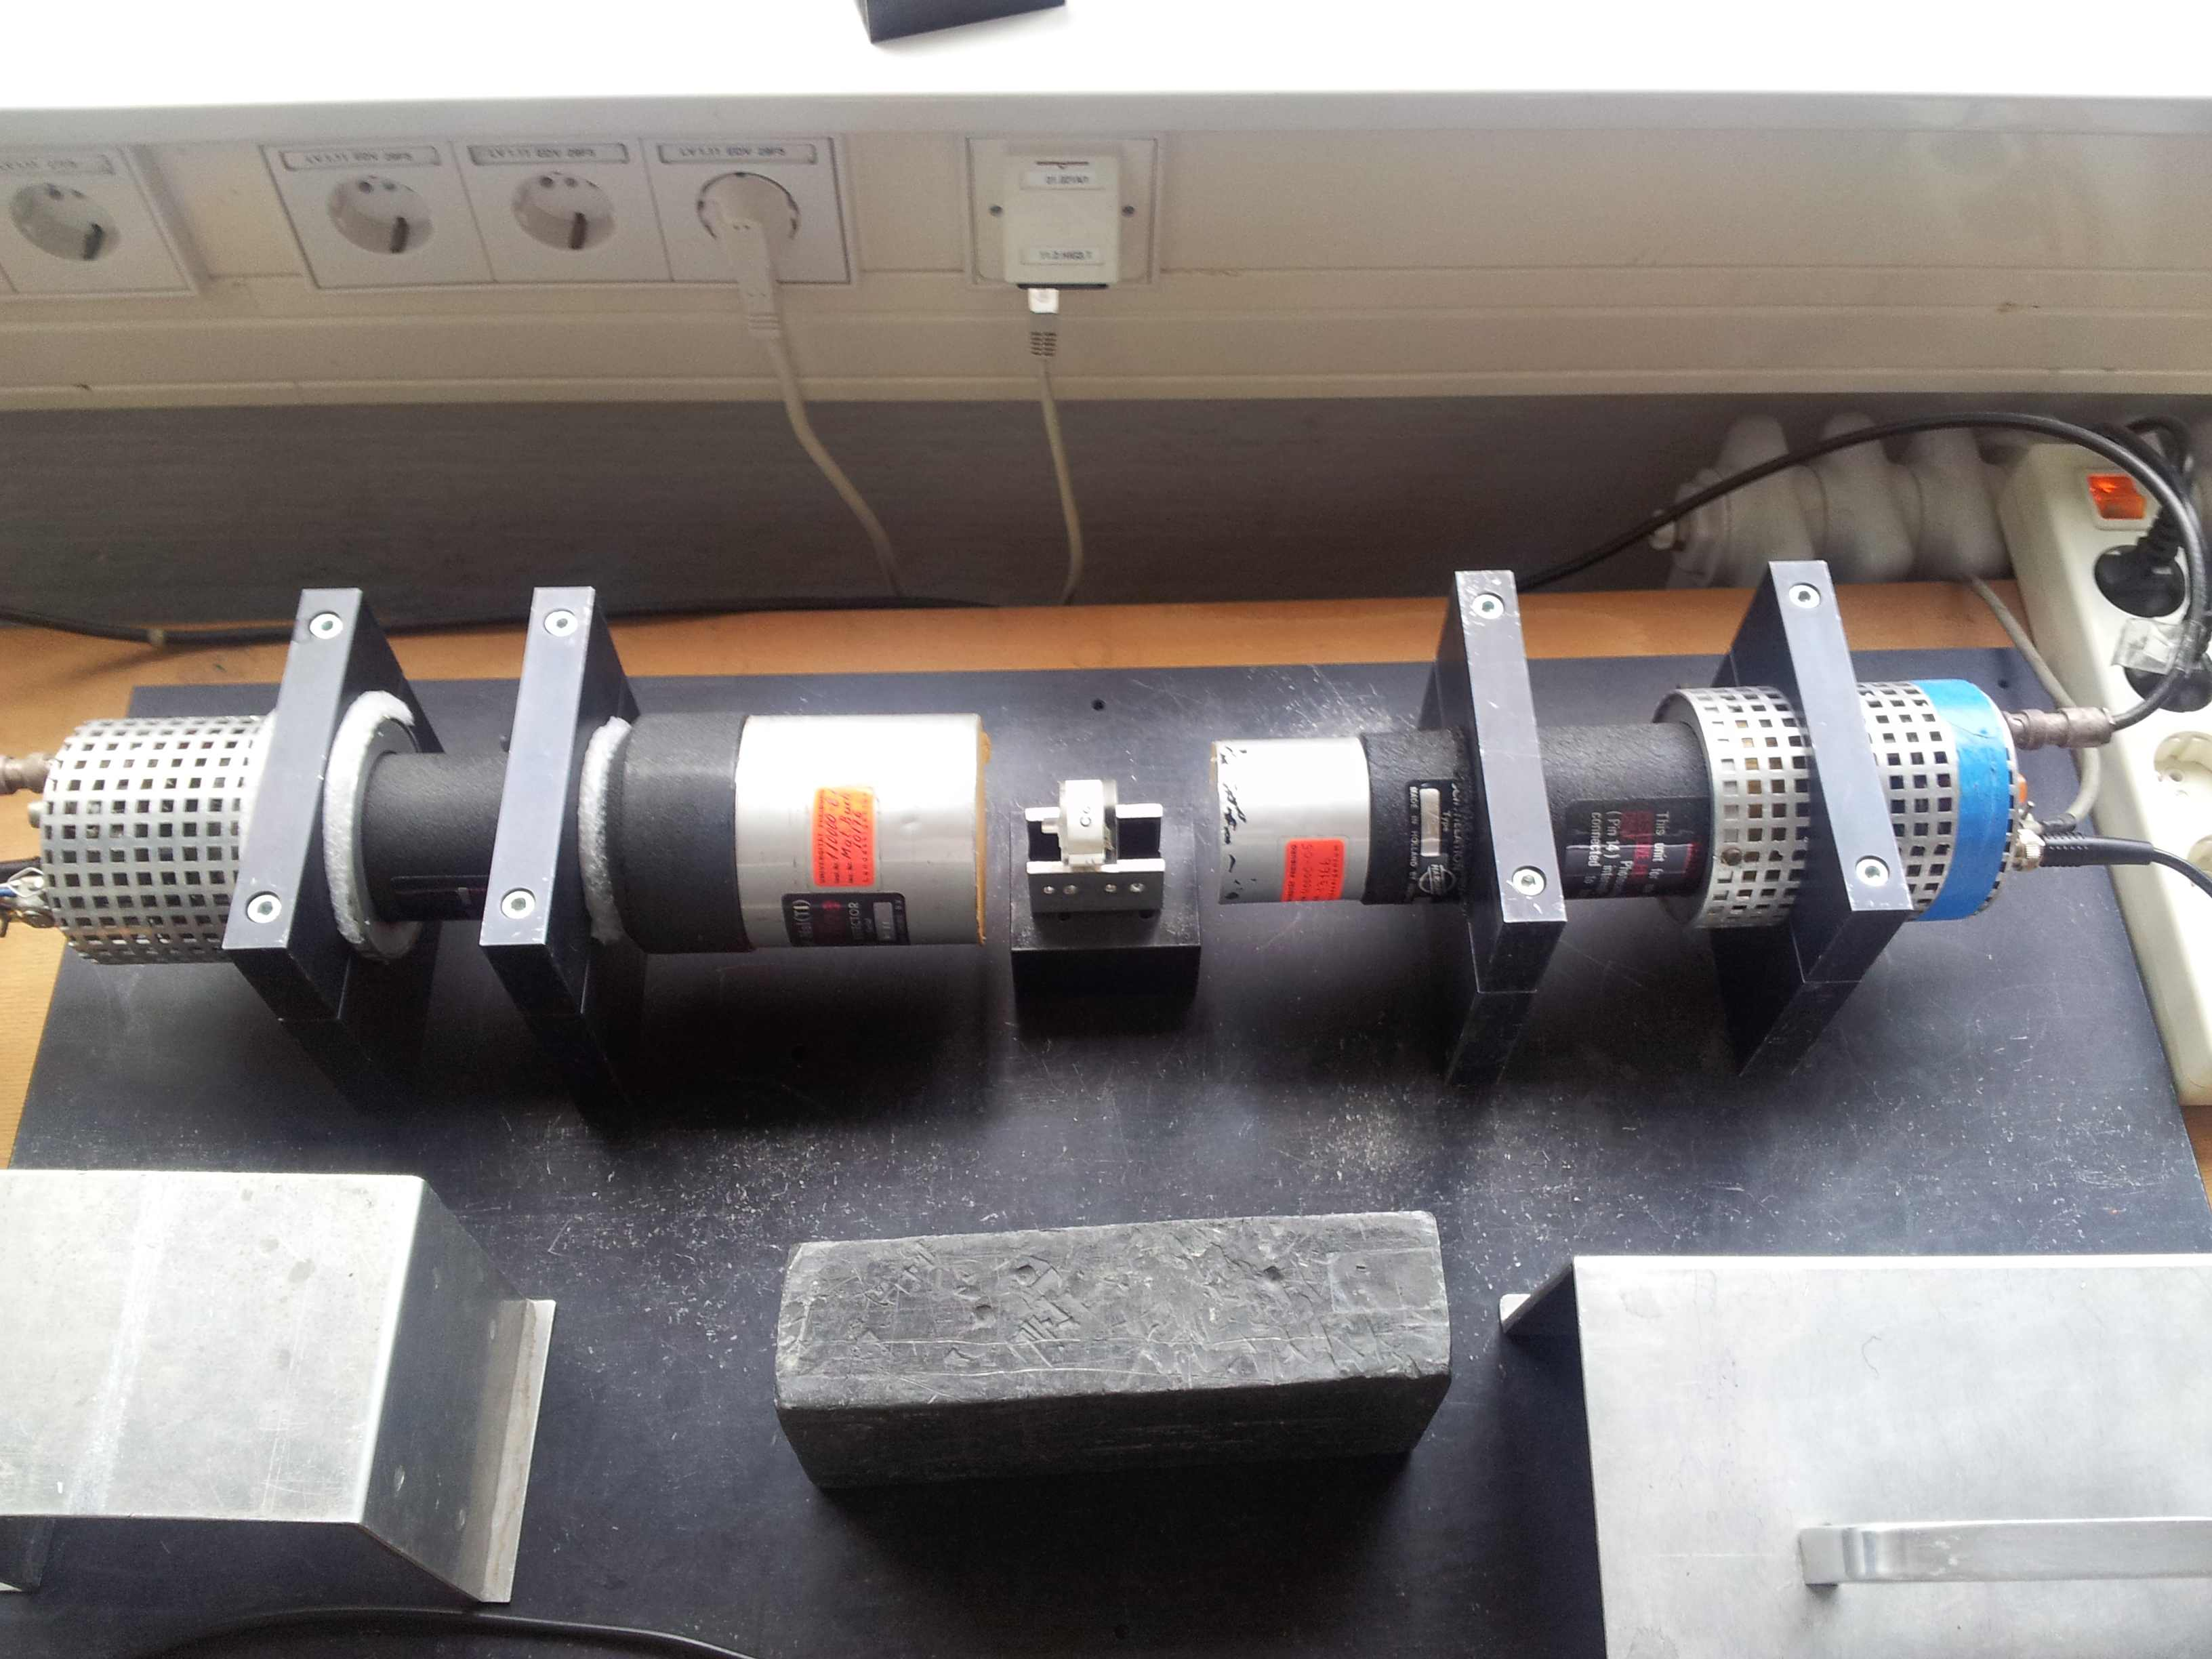
\includegraphics[width=0.8\linewidth]{figures/position_1.jpg}
    \caption{
        Photo of the $57$^Co probe and the two detectors with the setup used in the 
        experiment. The orientation of the probe is the one used for the measurement of 
        the delayed coincidences, with the larger opening facing the right detector. 
        During the measurements, the probe is isolated by the 
        }
    \label{fig:position_1}
\end{figure}




\clearpage

\section{Bibliography}
\printbibliography[heading=subbibintoc,type=article,title={Articles only}]
\printbibliography[heading=subbibintoc,type=book,title={Books only}]


\end{document}
